\documentclass[a4paper]{article}
\usepackage{amsmath}
\usepackage{graphicx}
\usepackage[margin=1in]{geometry}
\title{Swerve Drive}
\author{Yousuf Soliman\\Noah Sutton-Smolin\\Kian Sheik}
\begin{document}
\maketitle
\section{Introduction}
The drive train is one of the fundemental systems that a robot uses to move. There are countless different drive trains that robots could employ to maneuver. Most drive trains can fall under one of two distinct categories, \textbf{Omnidirectional} or \textbf{Standard}. 

Omnidirectional drive trains have the ability to move in any direction. Omnidirectional robots can simply move in any desired direction without the need to rotate, they can also employ more advanced techniques that allow a driver to control the Omnidirectional robot in relation to the field rather than in relation to the robot itself. In other words, it allows the driver to move the robot forward regardless of its orientation. 

When we look at the other class of drive trains, we can see that Standard drive trains cannot strafe and must rotate before moving in order to move to the side. The heading of these drive trains are modified through an arc. Standard drive trains do not have as much maneuverability as Omnidirectional systems, but they are much simpiler and \textit{generally} provide more torque and power. 
\subsection{An Overview of Several Drive Trains}
\begin{description}
\item[Differential] This is one of the simplest Standard drive trains. There are two sets of wheels on either side of the robot (left/right). When both sides spin in the same direction, the robot will move straight; however, if one side drives faster than the other side, the robot will move in an arc in the direction of the side that is moving slower. To turn in spot with a Differential drive train one set of wheels moves in one direction while the second set moves in the opposite direction. Wheels in a Differential drive train can often skip or skid. The greater the width of the robot, the less the skidding will occur. Differential drive trains only require two motors. Several subsets of Differential drive trains are West-Coast Drive and Tank Drive. 

\begin{figure}[h]%
\begin{center}
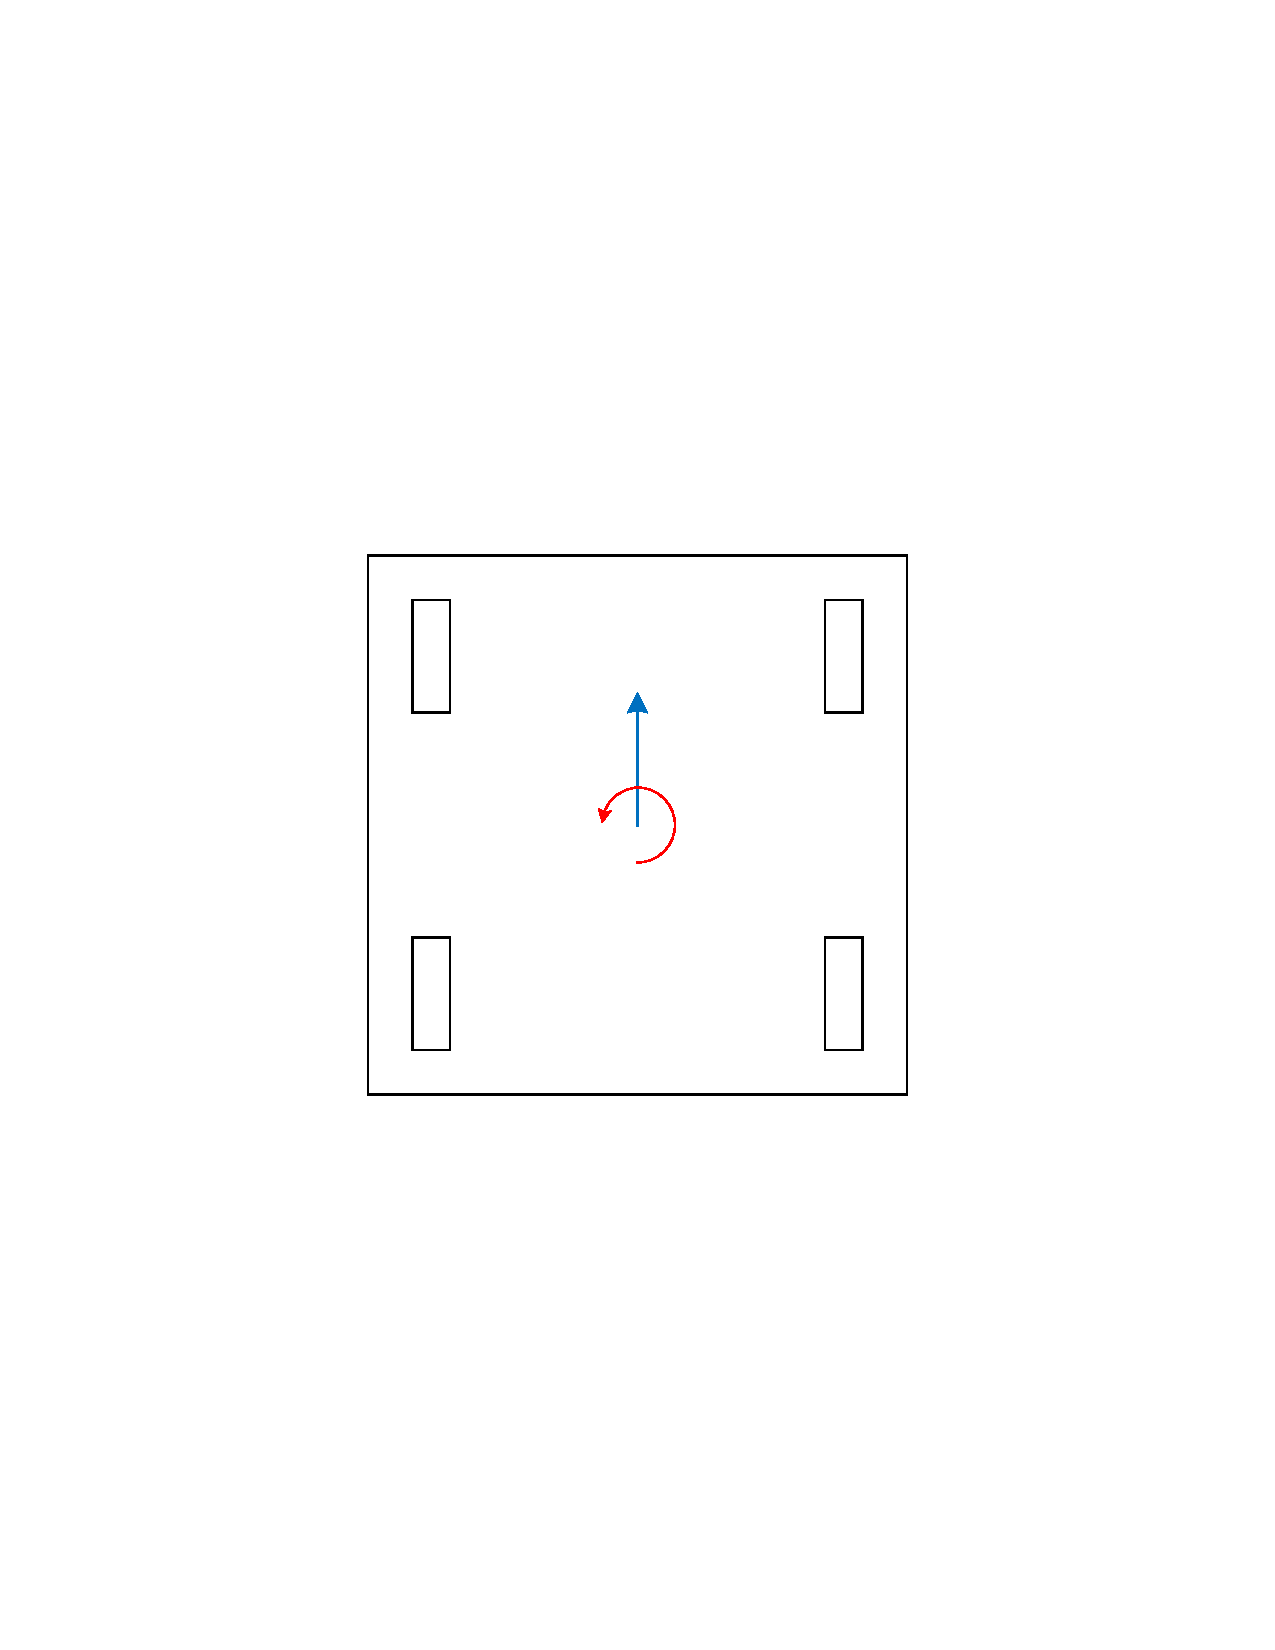
\includegraphics[scale=0.6]{Diagrams/DifferentialDrive.pdf}
\end{center}
\caption{A basic Differential drive train. It only has 2 axes of motion.}%
\label{DiffDrive}%
\end{figure}

\item[Ackerman] The Ackerman drive train, a Standard drive train, is one of the most widely used. It is often known due to its implementation in automobiles. The rear set of wheels is stationary and provides all of the power to the system. The front wheels provide the robot the ability to steer. If the front wheels slip at all, the ability of the robot to navigate is greatly negated. The Ackerman drive train is most beneficial when maneuverability is not a concern and the robot will be moving mostly straight with gentle turns. This is almost never the case and thus it is rarely found in the realm of robotics. Ackerman drive trains require one drive motor and one steering motor. 

\item[Holonomic] The Holonomic drive train is one of the more simple Omnidirectional systems. Its omnidirectional ability is achieved through the use of special wheels that have rotating ``mini rollers'' across the circumferance of the wheel. The rollers allow the side to side motion of the wheel. Each of the wheels is placed at either a $\pm 45^\circ$ angle at the corners of the robot. If we inscribe a circle within the perimiter of a square base, the wheels will be placed tangentially near the corners. This shape forms two distinct sets of parallel wheels which are perpendicular to each other. When all the wheels are powered the robot will spin around itself. When one set of wheels spin in the same direction the robot will move in that direction as the rollers on the other set will allow them to slide with the robot. This system provides outstandinding maneuverability in any plane. To achieve this, the Holonomic drive sacrifices torque and is easily pushed around. The Holonomic drive train requires a drive motor for each wheel. 
\end{description}

\begin{figure}[h]%
\begin{center}
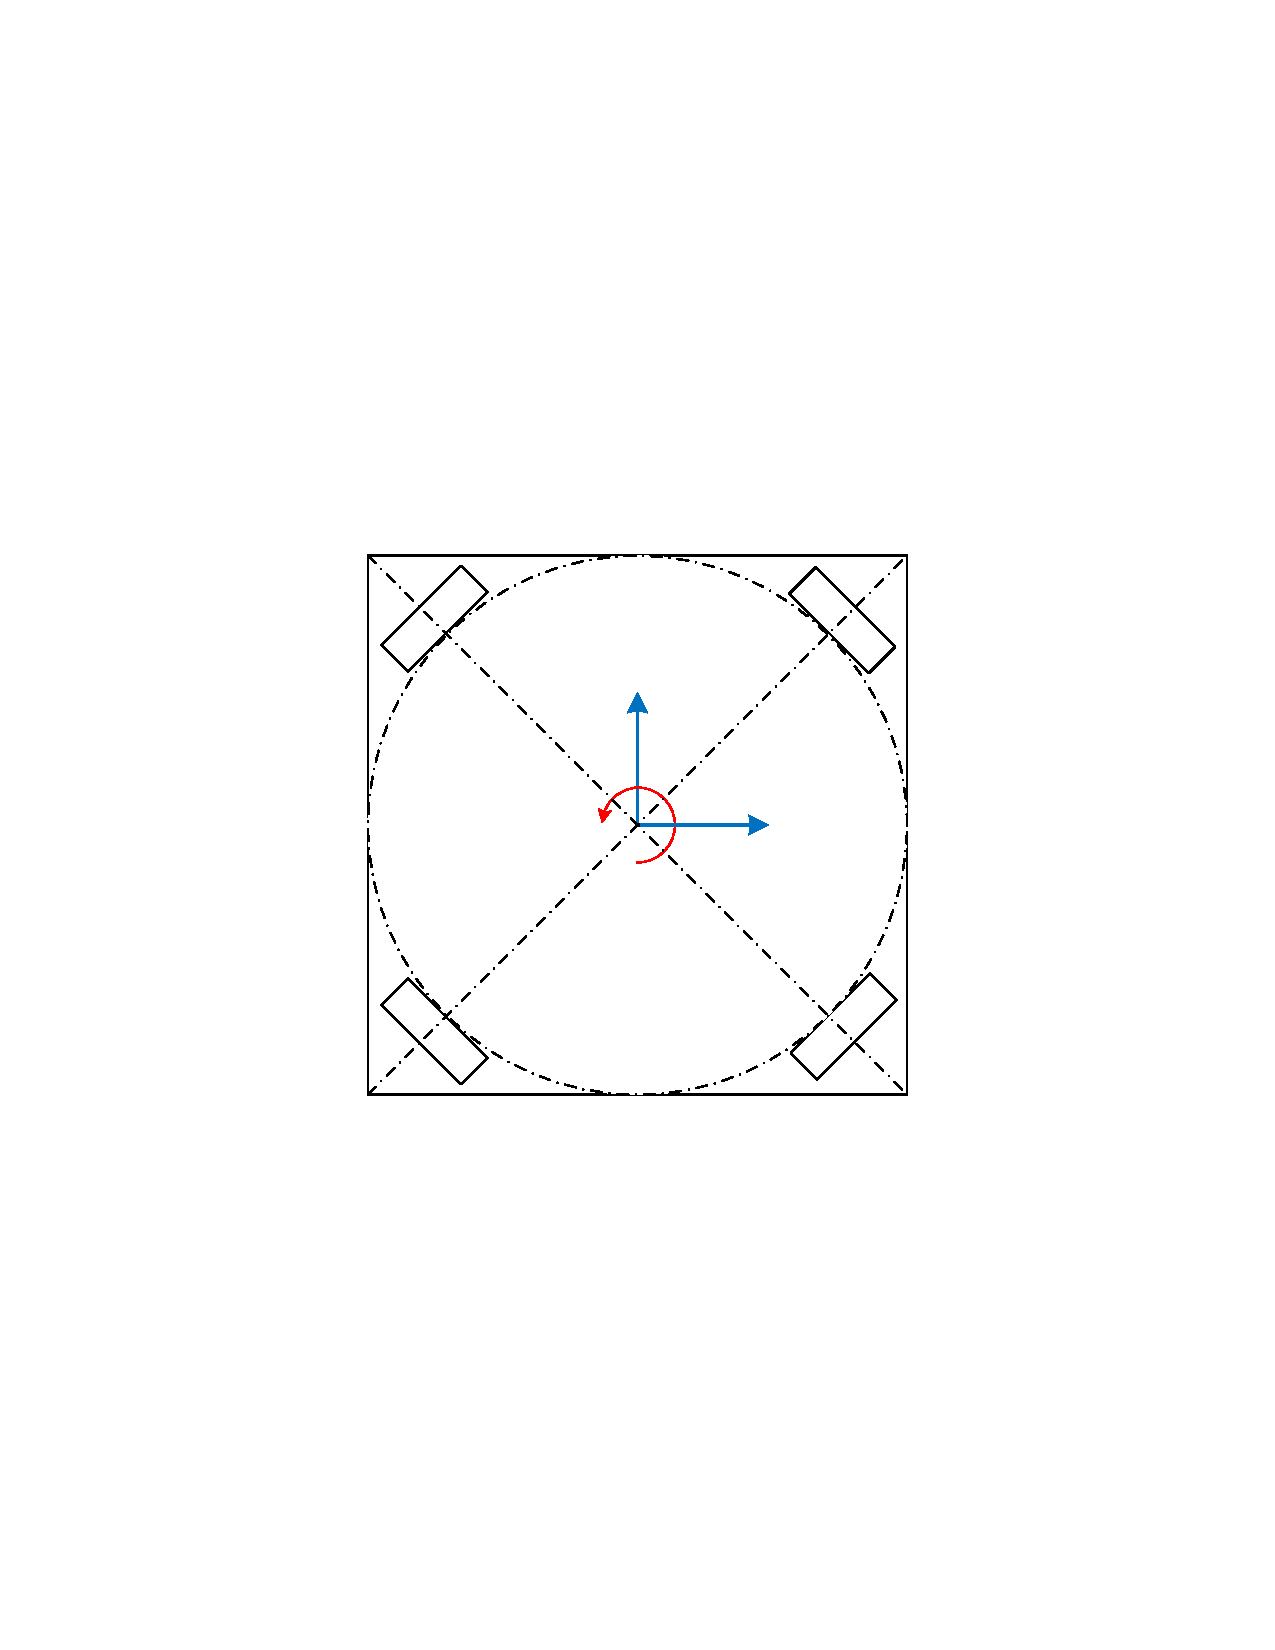
\includegraphics[scale=0.6]{Diagrams/HolonomicDrive.pdf}
\end{center}
\caption{A basic Holonomic drive train. It has 3 axes of motion}%
\label{HolDrive}%
\end{figure}
The following table provides an overview of the advantages and downsides to the drive trains discussed above: \newline \newline
\begin{tabular}{l|*{3}{l}}
Drive Train				& Pros & Cons \\
\hline
Differential 		& Simple, Durable, Light 		& Skids, Chassis Shape Restriction \\
Ackerman 				& Simple, Sturdy 						& Poor Maneuverability, Unable to Spin \\
Holonomic 			& High Maneuverability, Moderate Complexity		& High Cost, Low Traction 
\end{tabular}
\newline \newline \newline
The rest of the document will be dedicated to an understanding of the Swerve drive, both intuitively and mathematically. 

\section{Swerve Drive}
The Swerve Drive can be thought of as the holy grail of drive trains. It has the most maneuverability out of all of the available drivetrains and it can mimic any feature of any other drive train. Swerve Drive does \textit{everything}. The downside is that Swerve Drive is, by far, the most complex drive train to build and program. Swerve has at least twice the amount of moving parts and is relatively fragile. In almost every other drive train the wheels are bolted to the chassis, making it very robust. In a Swerve Drive, an impact to the wheels is not transmitted to a sturdy chassis, but rather to another moving part: the Swerve module. The Swerve system has many more points at which it could fail, but this is not to discourage you from implementing this drive train. It requires 4 drive motors and 4 motors for turning. 

\subsection{An Intuitive Explanation of Swerve Movement}
The Swerve Drive consists of $4$ motors which power the wheels and 4 motors which control their respective angles. Since each wheel has an independent power and rotation, we are now able to think about how this can work. By compounding each wheel's force vectors we can move the robot. For example, right side movement is possible with rotating the angles of all the wheels to $+90^\circ$ and rotating them in the forward direction. Similarly, forward right diagonal side movement is possible with rotating all wheels to $+45^\circ$ and forward rotating them. 

\subsection{A Mathematical Approach to Understanding the Swerve Drive}
For any arbitrary motion, the calculations of each weel is relatively simple as follows: 
\begin{align*}	\vec v_R &= \vec v +\vec \omega\times\vec r_R \\
								\vec v_L &= \vec v +\vec \omega\times\vec r_L \end{align*}
and in Cartesion form:
\begin{align*} 	v_{R_x}	&=v_x-\omega b \\ 
								v_{R_y} &=v_y+\omega a \\
								&\\
								v_{L_x}	&=v_x-\omega b \\
								v_{L_y}	&=v_y-\omega a	\end{align*}
								
It is then theoretically simple to convert the Cartesian vectors representing the velocities of each wheel into polar vectors. These polar vectors can then be directly used to control each wheel's speed and orientation. 

\begin{figure}[h]%
\begin{center}
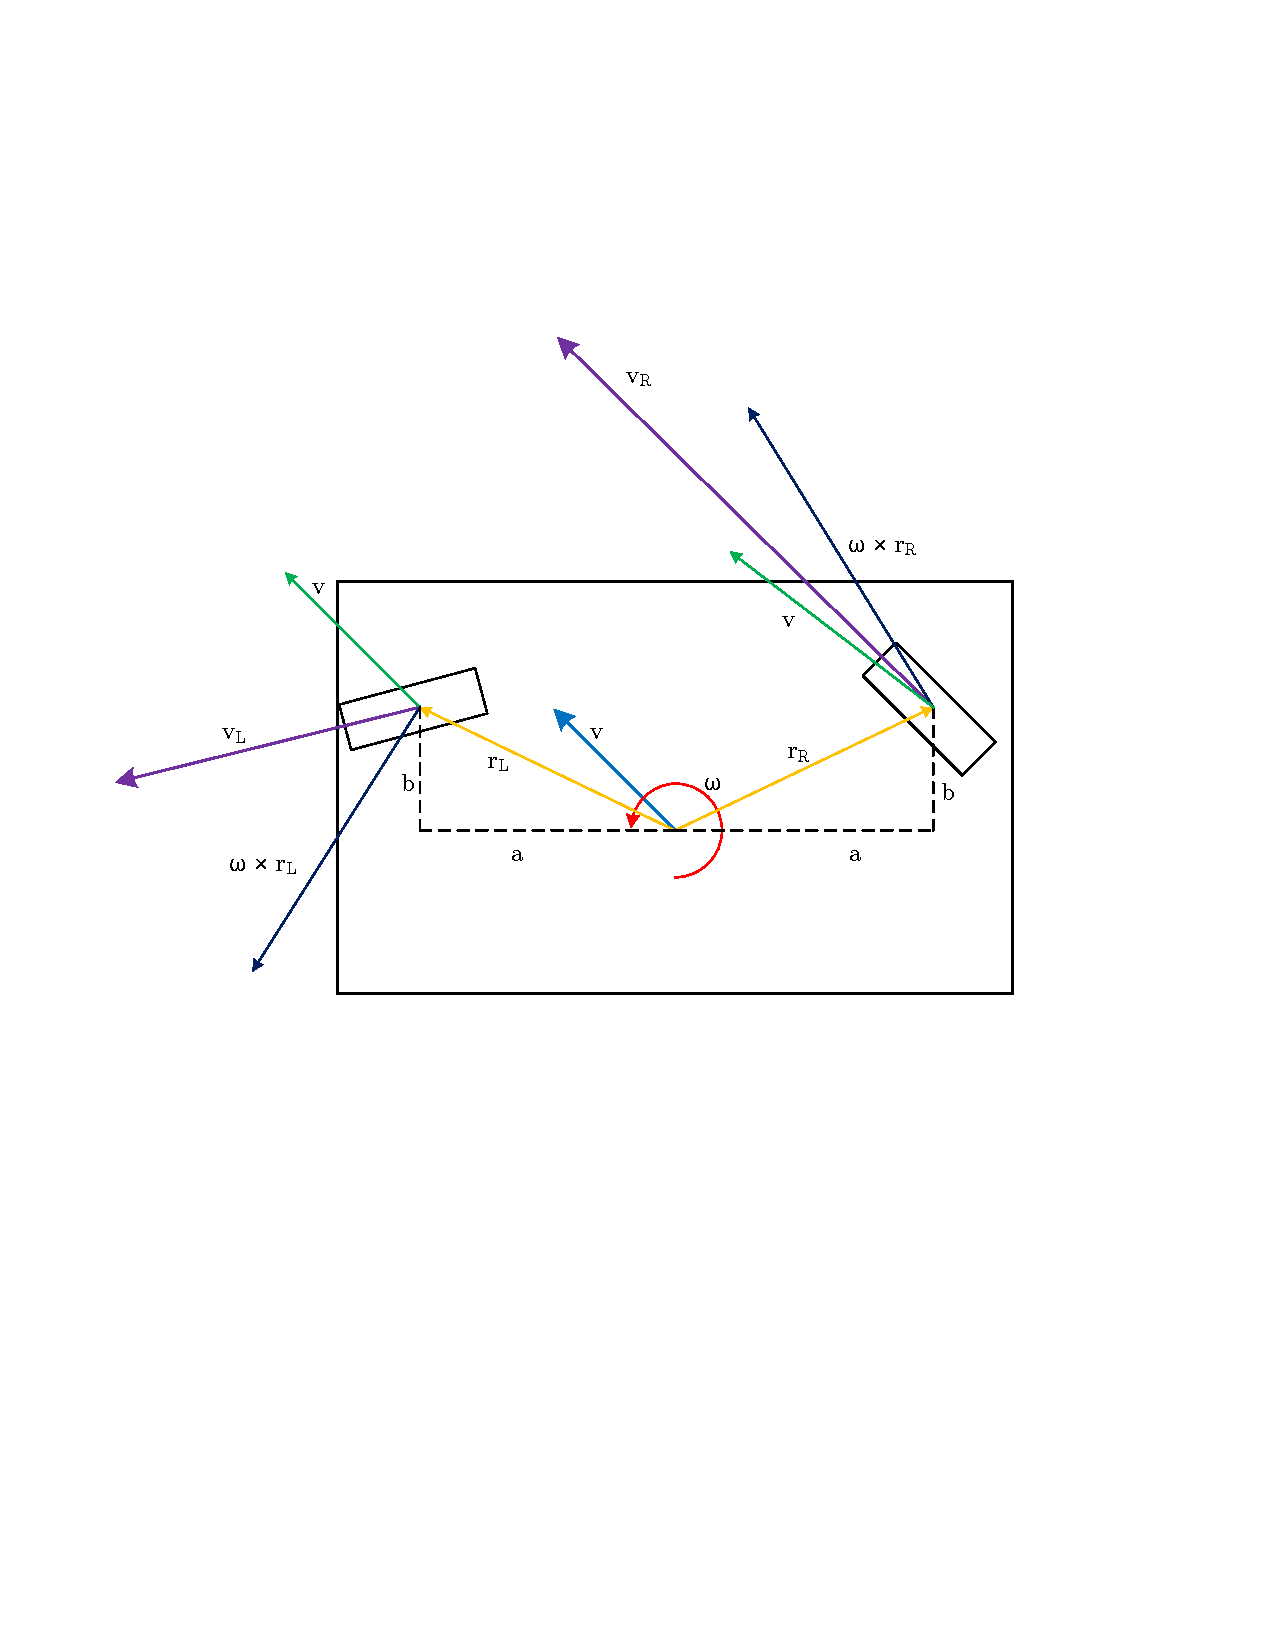
\includegraphics[scale=0.9]{Diagrams/SwerveMath.pdf}
\end{center}
\caption{A visualization of the Swerve theory}%
\label{SwerveMath1}%
\end{figure}

We can go further and do the calculations for all 4 wheels as follows:
\begin{align*}	v_{R_{x1}}	&= v_{x}-\omega  \\
								v_{R_{y1}}	&= v_{y}+\omega  \\
								&\\
								v_{R_{x2}}	&= v_{x}+\omega  \\
								v_{R_{y2}}	&= v_{y}+\omega  \\
								&\\
								v_{L_{x1}}	&= v_{x}-\omega  \\
								v_{L_{y1}}	&= v_{y}+\omega  \\
								&\\
								v_{L_{x1}}	&= v_{x}+\omega  \\
								v_{L_{y1}}	&= v_{y}-\omega  \\ \end{align*}
								
\begin{figure}[h]%
\begin{center}
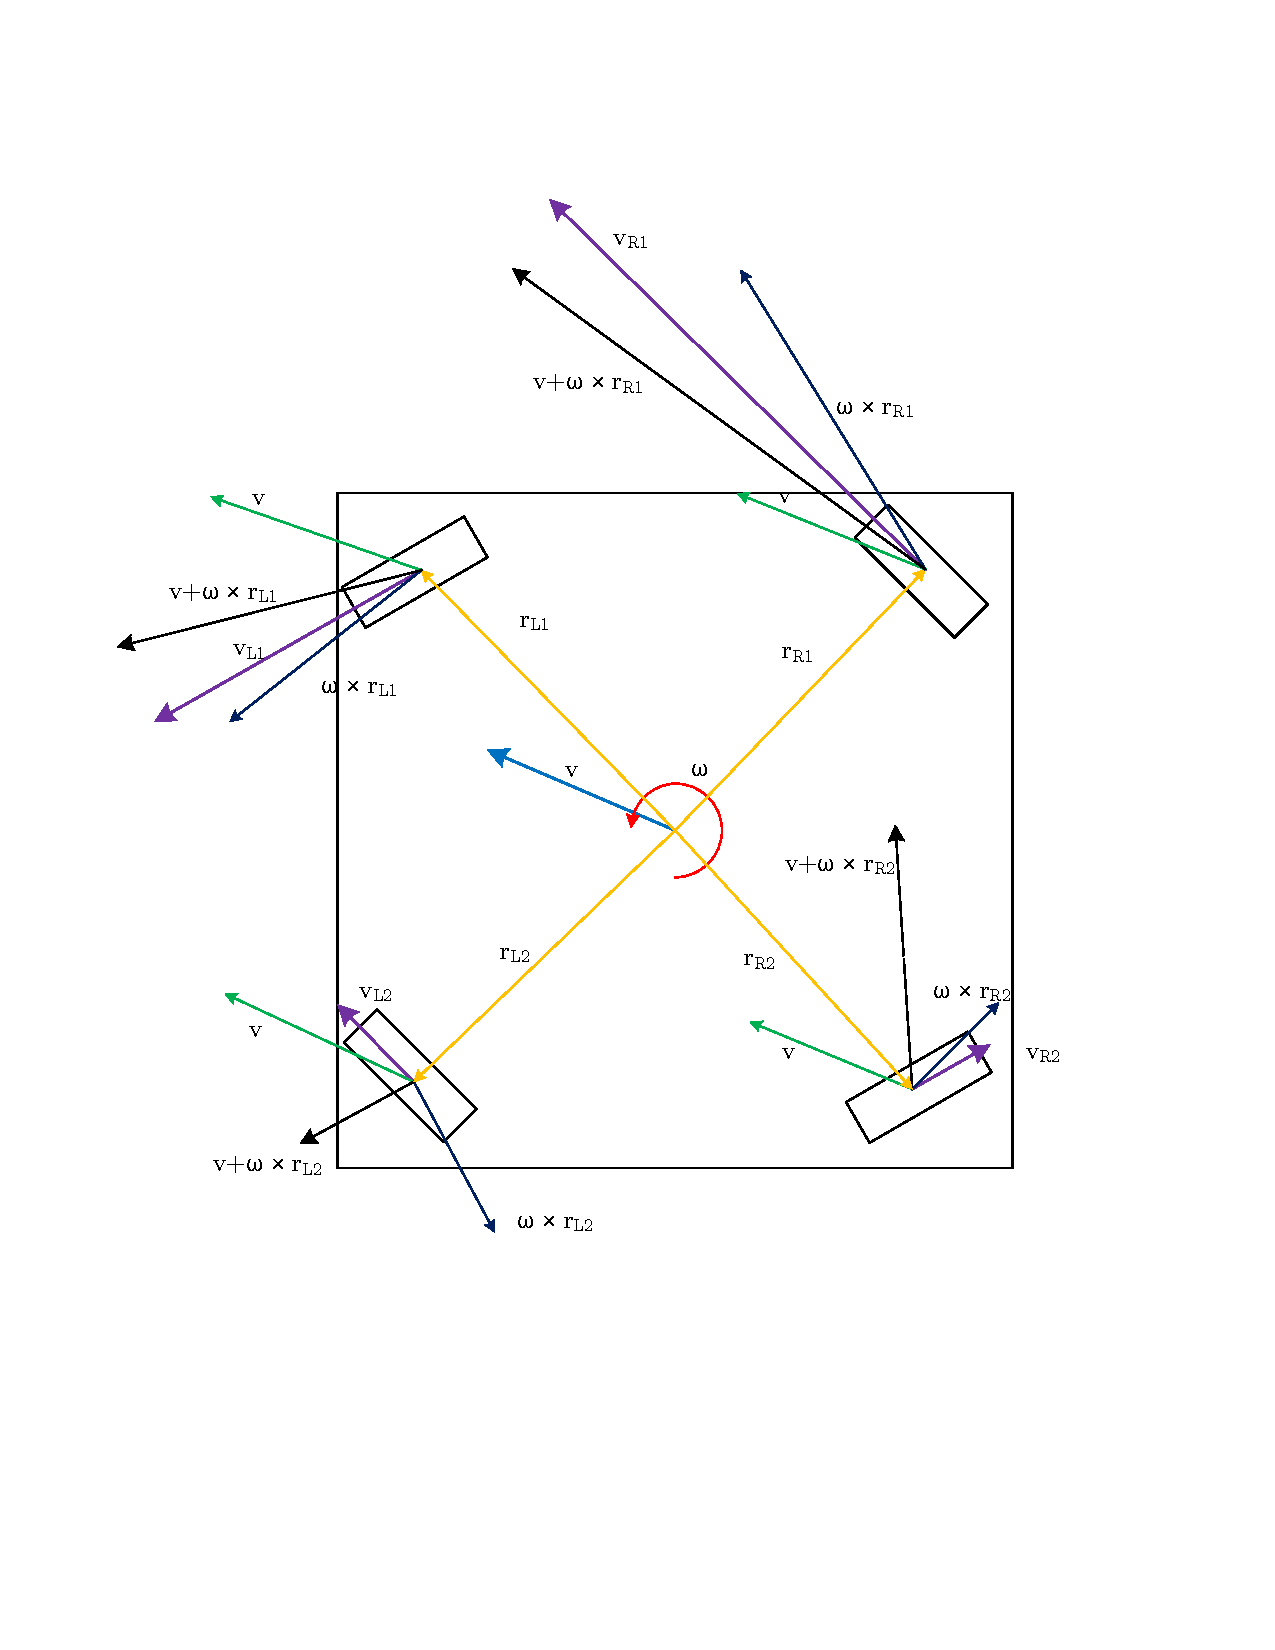
\includegraphics[scale=0.7]{Diagrams/SwerveMathExtensive.pdf}
\end{center}
\caption{A full visualization of a Swerve drive}%
\label{SwerveMathExtensive}%
\end{figure}

It should be noted that there is another method for omnidirectional drive that does not rely on wheels that can change direction (e.g. Holonomic or Mechanum).

Notice that the swerve drive can be completed with 2 wheels that have full \textit{independent} rotation and power controls. We will now go on to solve the generalized Swerve algorithm for $n$-Wheels. 
\newpage

\subsection{$n$-Wheel Swerve}
Let us first begin by picking a fixed point $C$ on the robot as the reference for all of the calculations. 

Fix the $xy$-Cartesian coordinate system onto the robot with the orgin at $C$ and the positive $y$-axis pointing in the robots forward direction. 

We will denote the position of the $i^\text{th}$ Swerve module by the coordinates $(x_i,y_i)$ and the desired clockwise robot rotation in radians/second about the point $C$ by $\omega$. Let $\vec v$ be the velocity vector. 

The forward speed of the $i^\text{th}$ wheel should be set to: $$v_i=\sqrt{\left(v_x+\omega y_i\right)^2+\left(v_y-\omega x_i\right)^2}$$
and the angle, $\theta_i$, should be set to: $$\theta_i=\frac{180}{\pi}\tan^{-1}\left(\frac{v_x+\omega y_i}{v_y-\omega x_i}\right)$$
For all of this to work, the velocity units must be consistent with distance units. If any of the $n$-Wheels exceeds the maximum, scale all wheel speeds down by the same factor. 
\end{document}
